\section{Programmable Storage}
\label{sec:progly}

The most common approaches for designing workarounds capable of handling application requirements not met by an underlying storage system roughly fall into among three categories:

{\bf Extra services.} ``Bolt-on'' services are intended to improve performance
or enable a feature, but come at the expense of additional hardware, software
sub-systems, and dependencies that must be managed, as well as trusted.
For instance, such classes of limitations inspired many extensions to Hadoop
~\cite{bu:vldb2010-haloop, ekanayake:hpdc2010-twister,
ekanayake:escience2008-eglmapreduce, mihailescu:hotstorage2012-mixapart}.

{\bf Application changes.} Changing the underlying application with the addition of
 more data management intelligence or via the integration of domain-specific middleware
 represents another popular option for adapting to storage system deficiencies. 
 When application adjustments depend on non-standard semantics exposed by the storage
system (e.g. relaxed POSIX file I/O or MPI-IO hints) the resulting coupling 
can be fragile.
For example, both SchiHadoop~\cite{buck:hpc2011-scihadoop} and Rhea~\cite{gkantsidis:nsdi2013-rhea} do
an excellent jobs of partitioning data in Hadoop applications, but may not
withstand the test of time for future workloads, since the partitioning is
specific to scientific data.

{\bf Storage modifications.} When these two approaches fail to meet an
application's needs, developers may turn their attention to any number of
heavyweight solutions ranging from changing the storage system itself, up to
and including designing entirely new systems. This approach can require
significant cost, domain knowledge, and extreme care when building or
modifying critical software that can take years of code-hardening to trust.
For example, HDFS fails to meet many needs 
of metadata-intensive workloads~\cite{shvachko:login2012-hdfs-scalability}.
Systems builder achieve performance improvement by modifying the underlying
architecture or API~\cite{balmin:sigmod2012-clydesdale}.

Rather than relying on storage systems to evolve or applications to
change, the ``Malacology Approach''
manifests a hybrid technique which embraces interface instability without placing
an unmanageable burden on developers.

\subsection{The Malacology Approach}

%\textcolor{red}{HELP! We can't decide if this section should be called ``The
%Programmable Storage Approach" or ``The Malacology Approach" -- I argue that
%Malacology is the prototype but Noah thinks Malacology Approach makes more
%sense.}

Programmable storage systems improve the development experience over the lifecycles of long-lived and co-designed applications
and storage systems by exposing a number of existing internal services capable of principled composition. Importantly, the compositionality of the internal functionality aids in the development of higher-level application specific services~\cite{sevilla:eurosys17}.
Figure~\ref{fig:malacology} shows the architecture of Malacology, a prototype programmable storage system
implemented in Ceph, which exposes a variety of low-level internal services
such as custom object interfaces, cluster metadata management, and
load-balancing. While Ceph natively exposes file, block, and object
abstractions, Malacology demonstrates the construction of two real-world
services (ZLog~\cite{watkins:ucsc-soe-16-12} and Mantle~\cite{sevilla:sc15-mantle}) using only the composition of existing interfaces present in Ceph.

\begin{figure}[t]
\centering
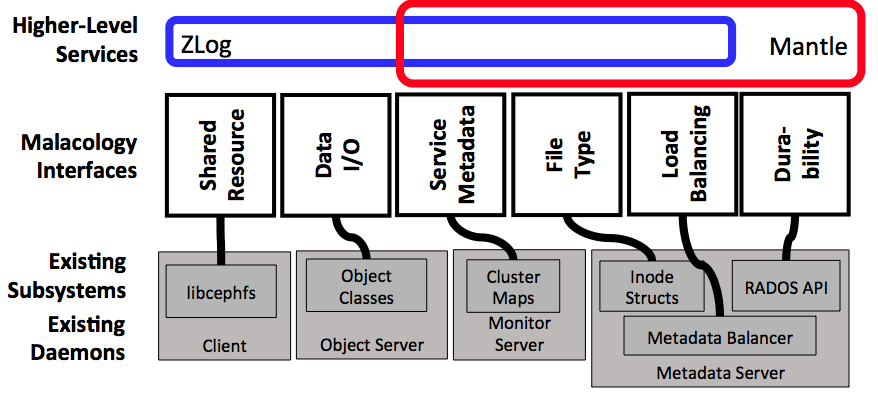
\includegraphics[width=1.0\linewidth]{implementation-overview.png}
\caption{Malacology implementation in Ceph. Existing sub-systems are composed
    to form new services and application-specific optimizations.}
\label{fig:malacology}
\end{figure}

ZLog is a high-performance distributed shared
log that implements the CORFU protocol~\cite{balakrishnan:nsdi12}.
This protocol achieves high-throughput by using a soft-state network-attached
counter and stripes log content over a cluster of flash devices exposing
protocol-specific storage interfaces. While CORFU is a stand-alone system,
Malacology is able to instantiate the same abstraction and approximate 
the same unique optimizations.

Malacology reproduces the CORFU network-attached counter service using a
capability-based mechanism found in the Ceph distributed file system for
managing cached metadata. ZLog implements the counter using the metadata server's ability to provide temporary
exclusive access to a shared resource (in this case, file metadata).  In ZLog, CORFU's storage device interface is
constructed using application-specific object interfaces in Ceph. These
software-based interfaces are constructed as a composition of low-level I/O
interfaces (e.g. an LSM-tree and a bytestream) operating in an atomic
context. The technique allows the interface to maintain consistency across native
interfaces.

The demonstration of interface synthesis in Malacology suggests a new form of
application development capable of significantly reducing the number of lines of code associated with a higher-level application.
While such an ability to construct software-defined interfaces is powerful,
subsequent analyses demonstrate how access to low-level interfaces can be a double-edged
sword providing extended application development powers at the cost of increased maintenance complexity.
